\documentclass[12pt]{book}

\usepackage{amsmath}
\usepackage{hyperref}
\usepackage{color}
\usepackage{enumerate}
\usepackage{fancyhdr}
\setlength{\headheight}{30pt}


\setlength{\oddsidemargin}{0cm}
\setlength{\evensidemargin}{0cm}
\setlength{\textwidth}{6.5in}
\setlength{\topmargin}{-2cm}
\setlength{\textheight}{9in}
 \pagestyle{plain}
\pagestyle{fancyplain}
\fancyhf{}
\lhead{ \fancyplain{}{ABC Player} }
\rhead{ \fancyplain{}{Andrei Ivanov, Olga Shestopalova, Zeke Schmois} }
\rfoot{ \fancyplain{}{\thepage} }

\renewcommand{\arraystretch}{1.5}	
\newcommand{\Ri}{\ \Rightarrow\ }
\newcommand{\Le}{\ \Leftarrow\ }
\newcommand{\Lr}{\ \Leftrightarrow\ }
\newcommand{\ds}{\displaystyle}
\newcommand{\ts}{\textstyle}
\newcommand{\sst}{\scriptstyle}
\newcommand{\sss}{\scriptscriptstyle}
\newcommand{\q}{\quad}
\newcommand{\ap}{\alpha}
\newcommand{\ii}{\^{\i}n }
\newcommand{\si}{\c{s}i }
\newcommand{\oaf}{oricare ar fi }
\newcommand{\nn}{\mathbb{N}}
\newcommand{\ns}{\mathbb{N}^{*}}
\newcommand{\rr}{\mathbb{R}}
\newcommand{\rs}{\mathbb{R}^{*}}
\newcommand{\cc}{\mathbb{C}}
\newcommand{\zz}{\mathbb{Z}}
\newcommand{\zs}{\mathbb{Z}^{*}}
\newcommand{\qq}{\mathbb{Q}}
\newcommand{\qs}{\mathbb{Q}^{*}}
\newcommand{\g}{\mathbb{G}}
\newcommand{\di}{\displaystyle}
\newcommand{\ai}{astfel \^{\i}nc\^{a}t }
\newcommand{\la}{\lambda}
\newcommand{\s}{\sigma}
\newcommand{\ri}{\ \rightarrow\ }
\newcommand{\gr}{^{\circ}}
\usepackage{graphicx}


\begin{document}
%%%%%%%%%%%%%%%%%%%%%%%%%%%%%%%%%%%%
%%%%%%%%%%%%%%%%%%%%%%%%%%%%%%%%%%%%
%%%%%%%%%%%%%%%%%%%%%%%%%%%%%%%%%%%%
%%%%%%%%%%%%%-------1------%%%%%%%%%%%%%%%%%
%%%%%%%%%%%%%%%%%%%%%%%%%%%%%%%%%%%%
%%%%%%%%%%%%%%%%%%%%%%%%%%%%%%%%%%%%
%%%%%%%%%%%%%%%%%%%%%%%%%%%%%%%%%%%%
%%%%%%%%%%%%%%%%%%%%%%%%%%%%%%%%%%%%
\phantom{xxx}
\bigskip
\centerline{{\large \bf Design Description }}
\bigskip\bigskip

We represent ???add some bullshit???

\centerline{ 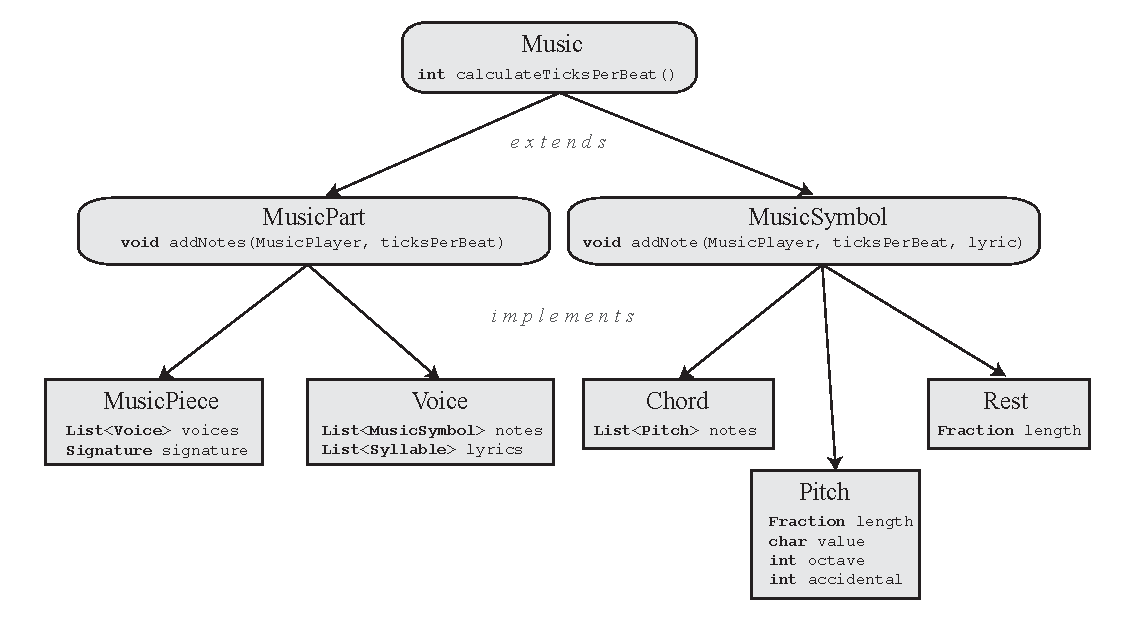
\includegraphics{Music.pdf}}

\noindent {\tt Music} is an interface that will represent our ADT. It defines the following method

\begin{itemize} 
\item { \tt calculateTicksPerBeat} is an auxiliar method needed to determine the number of ticks per beat for the player such that any notelength can be represented as an integer number of ticks. The method is called recursively.
\end{itemize}

\medskip 

\noindent {\tt MusicPart} is an interface that extends {\tt Music} and represents either a {\tt MusicPiece} or {\tt Voice}. It defines a method
\begin{itemize} 
\item { \tt addNotes} which takes an instance of  {\tt MusicPlayer} (described later) and adds to it all notes and lyrics found in the current {\tt MusicPart}  
\end{itemize}

\noindent and is implemented by the following classes:
\begin{itemize} 
\item { \tt MusicPiece} represents a final piece of music.   It has a {\tt signature} attribute which contains all the header information and {\tt List<Voice> voices} attribute which represents a list of different voices contained in this piece.
\item {\tt Voice}  represents a single voice in a piece of music. It has a {\tt List<MusicSymbol>notes } attribute which represents the sequence of notes the voice is made of and a  {\tt List<Syllable> lyrics } attribute that represents the lyrics that accompain the voice.
\end{itemize}

\bigskip

\noindent {\tt MusicSymbol} is another interface that extends {\tt Music} and represents either a {\tt Pitch}, a {\tt Rest} or a {\tt Chord}. It defines a method
\begin{itemize} 
\item { \tt addNote} which takes an instance of  {\tt MusicPlayer} and a lyric corresponding to the current symbol and modifies the player by adding notes and lyric to it. The  parameter {\tt ticksPerBeat} is used to convert the length of the note from a fraction to the number of ticks.
\end{itemize}

\noindent and is implemented by classes:
\begin{itemize} 
\item { \tt Pitch} represents a single pitch. Its attribute {\tt length} is represented by a fraction  of the length of the default note. The attribute {\tt value} is a pitch A,B,C,...,G from the middle octave,  {\tt octave} represents the offset from the middle octave and  {\tt accidental} is 1 for sharp and -2 for flat. Using these conviniences,  a {\tt Pitch} from out ADT can be easily converted to the {\tt Pitch} object described in the {\tt sound} package.
\item { \tt Rest} represents a single rest and has an attribute {\tt length}  represented by a fraction of the length of the default note. 
\item {\tt Chord} represents a chord of several pitches and stores them in the {\tt List<Pitch>} attribute.
\end{itemize}

These three basic music symbols let us implement any "musical expression" defined in the 6.005 subset. Any other structures like tuplets, triplets, repeats, etc. are converted to these basic music symbols during the ParseTree walk.  

\bigskip\bigskip


Another important class is a mutable {\tt MusicPlayer} which has two attributes 
\begin{itemize} 
\item { \tt player} that represents an instance of the {\tt SequencePlayer}. It collects the notes and lyrics of the song.
\item { \tt currentTick} which represents the current tick inside the player. It is used when the notes and lyrics are added consecutively to the player by the method {\tt addNote} to keep track of the position  where the notes need to be inserted. {\tt addNote} method increments it according to the length of the note.
\end{itemize}
It has the following methods:
\begin{itemize} 
\item { \tt addNote (int note, int numTicks)} that takes a converted Midi note and inserts it in the {\tt player} at the {\tt currentTick} position for a length of {\tt numTicks}.
\item { \tt addLyric (String Lyric)} that takes a syllable and adds it to the {\tt LyricListener} at the {\tt currentTicks} position.
\item { \tt addTime (int numTicks)} increases the {\tt currentTick} by {\tt numTicks}.
\item { \tt resetTime() } resets the {\tt currentTicks} to 0. This is used when starting a new voice.
\item { \tt play() } plays the notes and lyrics added.

\end{itemize}








\bigskip


      
      \end{document}
  

